\engchapter{Conclusions}
\section{Major Findings of the Study}
In this thesis, we analyzed the citation behaviors of 11 research papers written by distinct Chinese CS graduate students, in terms of citation quality, citation forms, and citation functions. We identified plagiarism and styling mistakes, and evaluated the quality of sources. The distribution of citations in terms of placement and function was analyzed, and speculations were proposed as an attempt to explain the differences with other studies. Examples were provided for each type of citation. We recorded the reporting verbs and signaling phrases the writers use when making citations. Moreover, how the writers used different citation functions were illustrated with examples.

\section{Limitations of the Study}

One major limitation of this study is the relatively small size of the dataset used. Only a number of 11 papers were studied, while one of them contains no citation at all, and another one is a review of recent literature rather than a typical research paper. For a qualitative case study purpose, these 9 valid samples could already serve as a miniature of Chinese CS graduate students’ research paper writing, and this analysis of citation behaviors could to some extent reasonably reveal the characteristics and limitations of Chinese CS graduate students. However, this sample size could not further support a solid and justifiable quantitative study, which would require datasets of a larger size to yield statistically significant quantitative findings.

In terms of methodology, this study only analyzed the research papers written by Chinese CS graduate students and made heuristic and preliminary comparisons with established findings and conclusions. Some researchers have conducted comparative studies that compared writers from different disciplines, or compared writings with different ratings (Hu \& Wang, 2014; Hyland, 2002; Mansourizadeh \& Ahmad, 2011; Petrić, 2007; Samraj, 2013). Some others have held interviews with the writers to investigate the hidden rationales of certain citation behaviors and the driving forces of a specific citation strategy (Fazel \& Shi, 2015; Harwood, 2009; Wette, 2017). Comparative studies would possibly help reveal the distinguishing citation behaviors of the certain group of writers, for example, Chinese CS graduate students, and interviews could facilitate the investigation of the latent factors that have caused the citation behaviors of Chinese CS graduate students.

This study used the original typology of citation functions of Petrić (2007), while more recent studies have adopted variations of Petrić’s typology with finer granularities and have introduced rhetorical moves into the typology (Fazel \& Shi, 2015; Mansourizadeh \& Ahmad, 2011). For example, they have extended the citation function \textit{Attribution} (to attribute a finding, proposition, theorem, hypothesis or method to an author) in Petrić’s original typology with rhetorical moves, specifically whether the writer is trying to provide background information, support the topic of the study, justify the procedures and materials, to support the writer’s claim, or to justify the findings (Mansourizadeh \& Ahmad, 2011), and in grant proposal writing to state the importance and potential benefit of the study or to show the competence of the writer (Fazel \& Shi, 2015). In our study, as many as 62\% of the citations identified were classified into the function \textit{Attribution}. The introduction of rhetorical moves would break down this type of citations to provide a clearer view of the citation behaviors, and may also help identify some common problems of novice academic writers, including using citations too often to supply content rather than support arguments as summarized by Wette (2017) and \textit{over-citation}, i.e. unnecessarily repeating the source (Davis, 2013; Petrić, 2012; Schmitt, 2007).

\section{Implications for Future Studies}
As summarized in Section 5.2, this study still contains limitations to which further studies could attend. Further studies could construct a larger dataset and apply methodologies and research paradigms similar to this study on it. Furthermore, quantitative methods could also be applied once there is a larger dataset. Researchers interested in the citation behaviors of Chinese CS graduate students may construct parallel datasets of high- and low-rated research articles to make comparative studies, or they may collect data from the same group of students in a chronological way to do longitudinal studies. External sources of information, including interviews of the student writers and detailed evaluations from professional EAP teachers could be added to the study design. In further studies, researchers may also investigate more detailed aspects of the citation behaviors of Chinese CS graduate students like rhetorical moves and investigate related mistakes of using citations, such as lack of supportive citations and over-citation.

\section{Possible Suggestions for EAP Teachers}

Before novice writers could play a significant role in academic communities, they have to move from a peripheral position to the center of academic communities by assimilating and demonstrating the shared practices of academic communities (Mansourizadeh \& Ahmad, 2011). Apparently, using citations is one of the shared practices of academic communities, and EAP teachers could help graduate students learn proper citation practices to fill the gap between a novice and a competent academic writer. Kwan \& Chan (2014) suggested that EAP teachers should conduct citation behavior analyses within each discipline and field to make their teaching more specific. For example, there are disciplinary differences in reporting verbs used (Davis, 2013), and teachers could incorporate disciplinary variations in their teaching. The findings of this study could serve this purpose by displaying the current status and major characteristics of Chinese CS graduate students’ citation use that teachers could refer to.

Only 11\% of the citations involve multiple sources, and therefore teachers may need to spend more energy in assisting students with their use of synthesizing, which is a complicated process (Bereiter \& Scardamalia, 2013; T. A. Hyland, 2009; Kirkland \& Saunders, 1991; Kwan \& Chan, 2014; Mayes, 1990; Segev-Miller, 2007) therefore is challenging to master. Davis (2013) stated that most teachers have adopted Swales’ (1990) Creating a Research Space (CARS) model, where the writers need to first synthesize and review multiple sources in order to establish a territory. The findings of this study suggest that additional emphases and training on synthesizing and reviewing multiple sources could be combined with the introduction of the Creating a Research Space model.

Regarding the mistakes in styling, teachers should instruct students to be aware of the disciplinary differences in style guides, and encourage them to get familiar with their own discipline. Samples of frequently made mistakes in citation style could be given to avoid the students making similar mistakes. Furthermore, there are various bibliography management software products available, such as EndNote, Zotero, and Mendeley, and recently they have been used prevalently in academic writing (Cuschieri, Grech, \& Calleja, 2019). In addition to managing all the literature stored in the computer, this type of software can help writers manage citations inside a document as well as generate a bibliography of all the works cited in the document that follows the citation and reference style configured. If the citation management job is delegated to bibliography management software, it would be less likely for writers to make mistakes in citation styles. Therefore, teachers could inform the students of the existence and capabilities of bibliography management software. For more information on prevalent bibliography management software and how to use them in academic writing, readers could refer to the work of Cuschieri, Grech, and Calleja (2019).

As shown by the analysis of the texts, when using citations some students are facing a language barrier to choose appropriate reporting verbs, phrases, and sentence structures. EAP teachers, especially teachers of L2 writers, might give explicit instructions and suggestions on useful reporting verbs and expressions. A feasible way is to help students organize reporting verbs and expressions based on Hyland’s (2002) taxonomy, as shown in Figure \ref{fig:taxonomy}. Hyland first classified reporting verbs into three categories in terms of the activities they refer to: research acts (to report procedures and findings that may be factive, counter-factive or non-factive), cognition acts (to evaluate), and discourse acts (to express attitudes). The acts can be further divided, for example cognition acts could be positive, critical, tentative, or neutral. Each leaf of the taxonomy tree corresponds to a set of verbs and phrases, for example, find, prove, show to report factive findings and fail to report counter-factive findings. Student writers could conveniently refer to this taxonomy to choose the proper words when writing research papers, and they can add new words and expressions to the taxonomy tree while reading to build up their vocabulary. Instructors could also inform students of the use of English writer’s thesauri to help them replace frequently used reporting verbs with their synonyms.

\begin{figure}[htb]
    \centering
    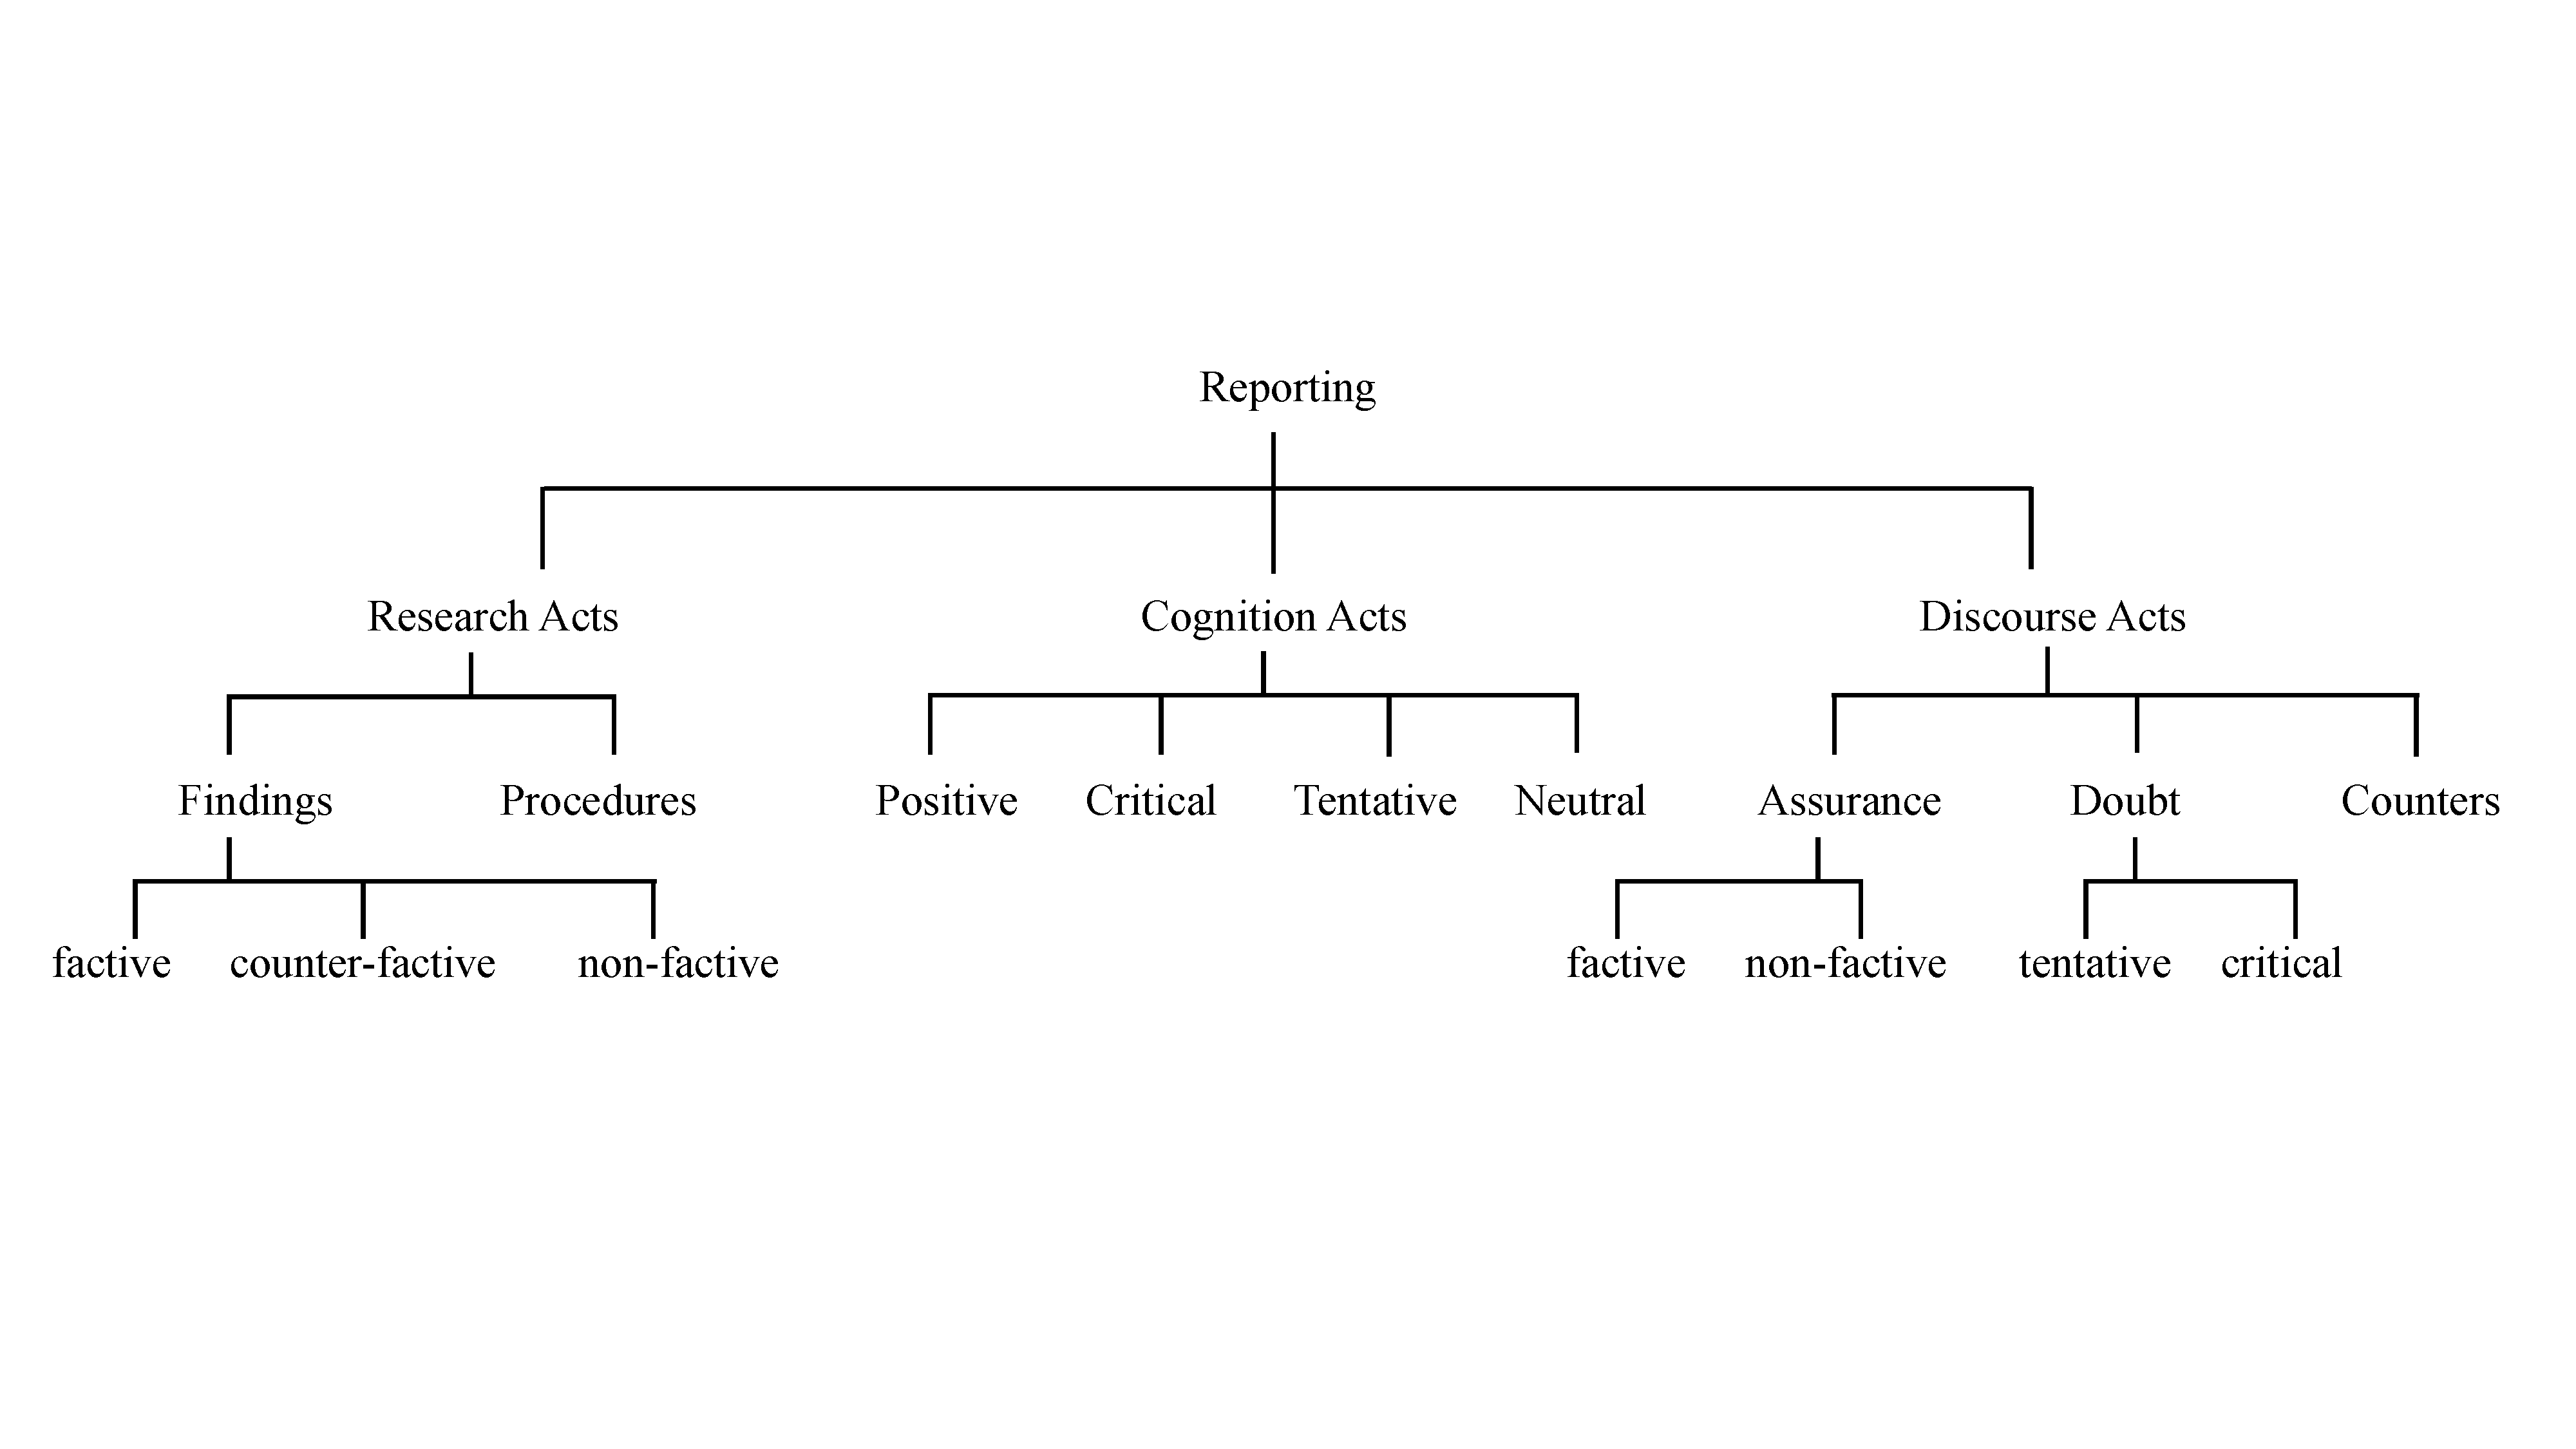
\includegraphics[width=\linewidth]{taxonomy}
    \caption[Hyland’s (2002) taxonomy of reporting verbs]{Hyland’s (2002) taxonomy of reporting verbs, reproduced from Peng’s (2019,  p.15) version.}
    \label{fig:taxonomy}
  \end{figure}

In general, several pedagogical implications on using citations pointed out by previous studies are also applicable in this study. For example, students should be informed of the different taxonomies of citations, i.e. how citations could be categorized into non-integral, integral (verb controlling), and integral (naming) in terms of form and what the different rhetorical functions or rhetorical moves of citations are (Kwan \& Chan, 2014; Mansourizadeh \& Ahmad, 2011). In the case of this study, teachers may instruct students that citations of type statement of use are often used when stating the datasets, software, and baseline models used, so that students might be less likely to make plagiarism like the case of TXT4 (missing citations for datasets and baseline models). In addition, teachers may identify research papers with proper citation use as examples and let students refer to them (Petrić \& Harwood, 2013; Ridley, 2006), or help students analyze the texts written by expert writers while highlighting on their citation use (Mansourizadeh \& Ahmad, 2011).